\section{Exploring Structure through Scattering}\label{ch1:sec1:background}

    %\subsection{Discovery of the Nucleons}
    The typical length scales for atoms and nucleons are 0.1 nm which is far smaller than the wavelength of human-visible light ($\sim$ 500 nm). As such, atomic and nuclear structure must be explored by forcing some interaction and then inferring the structure from the observed results. Thomson's atomic model was famously tested in the early 1900s by Ernest Rutherford's research group, wherein $\alpha$ particles were fired at thin metal targets, and the scattering behaviour was observed \parencite{Geiger1909OnAlpha-Particles} \parencite{Rutherford1911TheAtom}. 
    
    The results were not consistent with Thomson's model, but instead indicated that there was a very small, dense, positively charged nucleus at the center of every atom. Further experiments by Rutherford would lead to the discovery of the proton around 1920 \parencite{Rutherford1919CollisionNitrogen}. Puzzles about the nucleus remained, including a consistent description of isotopes, until 12 years later when James Chadwick suggested the existence of the neutron \parencite{Chadwick1932PossibleNeutron}. With electrons and the two nucleons discovered, it seemed as though the indivisible constituents of the atom were finally realized, but future experiments showed a much more complex, sub-nuclear structure. 
    
    \subsection{Scattering at Different Resolution Scales}

        The diffraction limit for microscopic (compared to telescopic) systems can be approximated by equation \ref{eq:diffraction}, where \textit{n} is the index of refraction, $\theta$ is a measure of the device aperture, $\lambda$ is the wavelength of the probe, and \textit{d} is the minimum resolvable length scale. Thus, the wavelength of a probe sets a fundamental lower limit on the achievable resolution of a microscopic imaging system - roughly, at small enough distances, the probe's waves interfer, prohibiting resolution at or below that scale. 
    
        \begin{equation}\label{eq:diffraction}
            d = \frac{\lambda}{2n\sin{\theta}}
        \end{equation}\myequations{ Diffraction Limit}
        
        For visible light microscope systems, $\lambda$ $\sim$ 500 nm, and so the minimum resolvable feature size is approximately \textit{d} $\sim$ 250 nm. Techniques exist to extend the resolution size by approximately an order of magnitude, e.g. expansion microscopy \parencite{Chen2015ExpansionMicroscopy} or Near-Field Scanning Optical Microscopy \parencite{Ma20216Source}, but non-visible-light probes are needed for scales below $\sim$ 10 nm. 

        
        %good guide: https://www.thermofisher.com/us/en/home/global/forms/industrial/backscattered-electrons-sem.html
        %Why no proton microscopes? https://physics.stackexchange.com/questions/574802/why-no-proton-microscopes-proton-diffraction-or-proton-scattering-experiments#:~:text=Proton%20crystallography%20is%20not%20typically,neutrons%20with%20the%20same%20energy.
        % Comprehensive book on electron microscopes: https://link.springer.com/book/10.1007/978-0-387-76501-3
        % Details on how to get beyond the diffraction limit with special tricks https://advanced-microscopy.utah.edu/education/super-res/

        In particular, the de Broglie relationship \ref{eq:deBroglie} \parencite{Broglie1924AQuanta} states that the wavelength $\lambda$ of a particle is inversely proportional to its momentum \textit{p}, with \textit{h} being Planck's constant. 
        
            \begin{equation}\label{eq:deBroglie}
               \lambda = \frac{h}{p}
            \end{equation}\myequations{ de Broglie Relationship}

        With this relationship, we can see that by increasing a particle's momentum, its effective wavelength is reduced. This is the fundamental principle which allows electron microscopes to image matter at a resolution of $\sim$ 10-0.1 nm \parencite{Franken2020ADevelopments}, corresponding to electron momentums of $\sim$ 1-100 keV. At this scale, viruses, cells, molecular structures, and even atoms can be imaged \parencite{Williams2009TransmissionMicroscopy}, with striking results commonly published online. Other probes could be used circumvent the diffraction limit, such as high energy (low-wavelength) photons or high momentum (low de Broglie wavelength) protons or neutrons, but electrons are an ideal candidate in this regime as they are easy to produce, steer, interact with, and detect. 

        To move beyond imaging at the atomic scale ($\sim$ 1 \AA) to the nuclear scale ($\sim$ 1 fm) requires probes that are 100,000 times more powerful. Electrons are still an ideal probe due to their (apparent) lack of internal structure, but rather than a room sized microscope, an entire accelerator facility is needed to achieve high enough energies and luminosities for sub-nuclear scale resolution. 
        


    \subsection{Elastic Scattering and Form Factors}

        Imaging with electrons (or other non-visible-light probes) at any energy scale is commonly understood in terms of scattering cross sections, $\sigma$, with dimensions of area and interpreted as the probability for a certain interaction to occur. Typical elastic scattering cross sections for transitions metals with 100 keV incident electrons as in electron microscopy are $\sim 10^{-22} m^2$ \parencite{Williams2009TransmissionMicroscopy}. In contrast, the cross sections to be discussed in this thesis are on the order of tens of nanobarn ( $10^{-36} m^2$), or 14 orders of magnitude smaller. 
        
       % \begin{figure}[h]
       %     \centering
      %      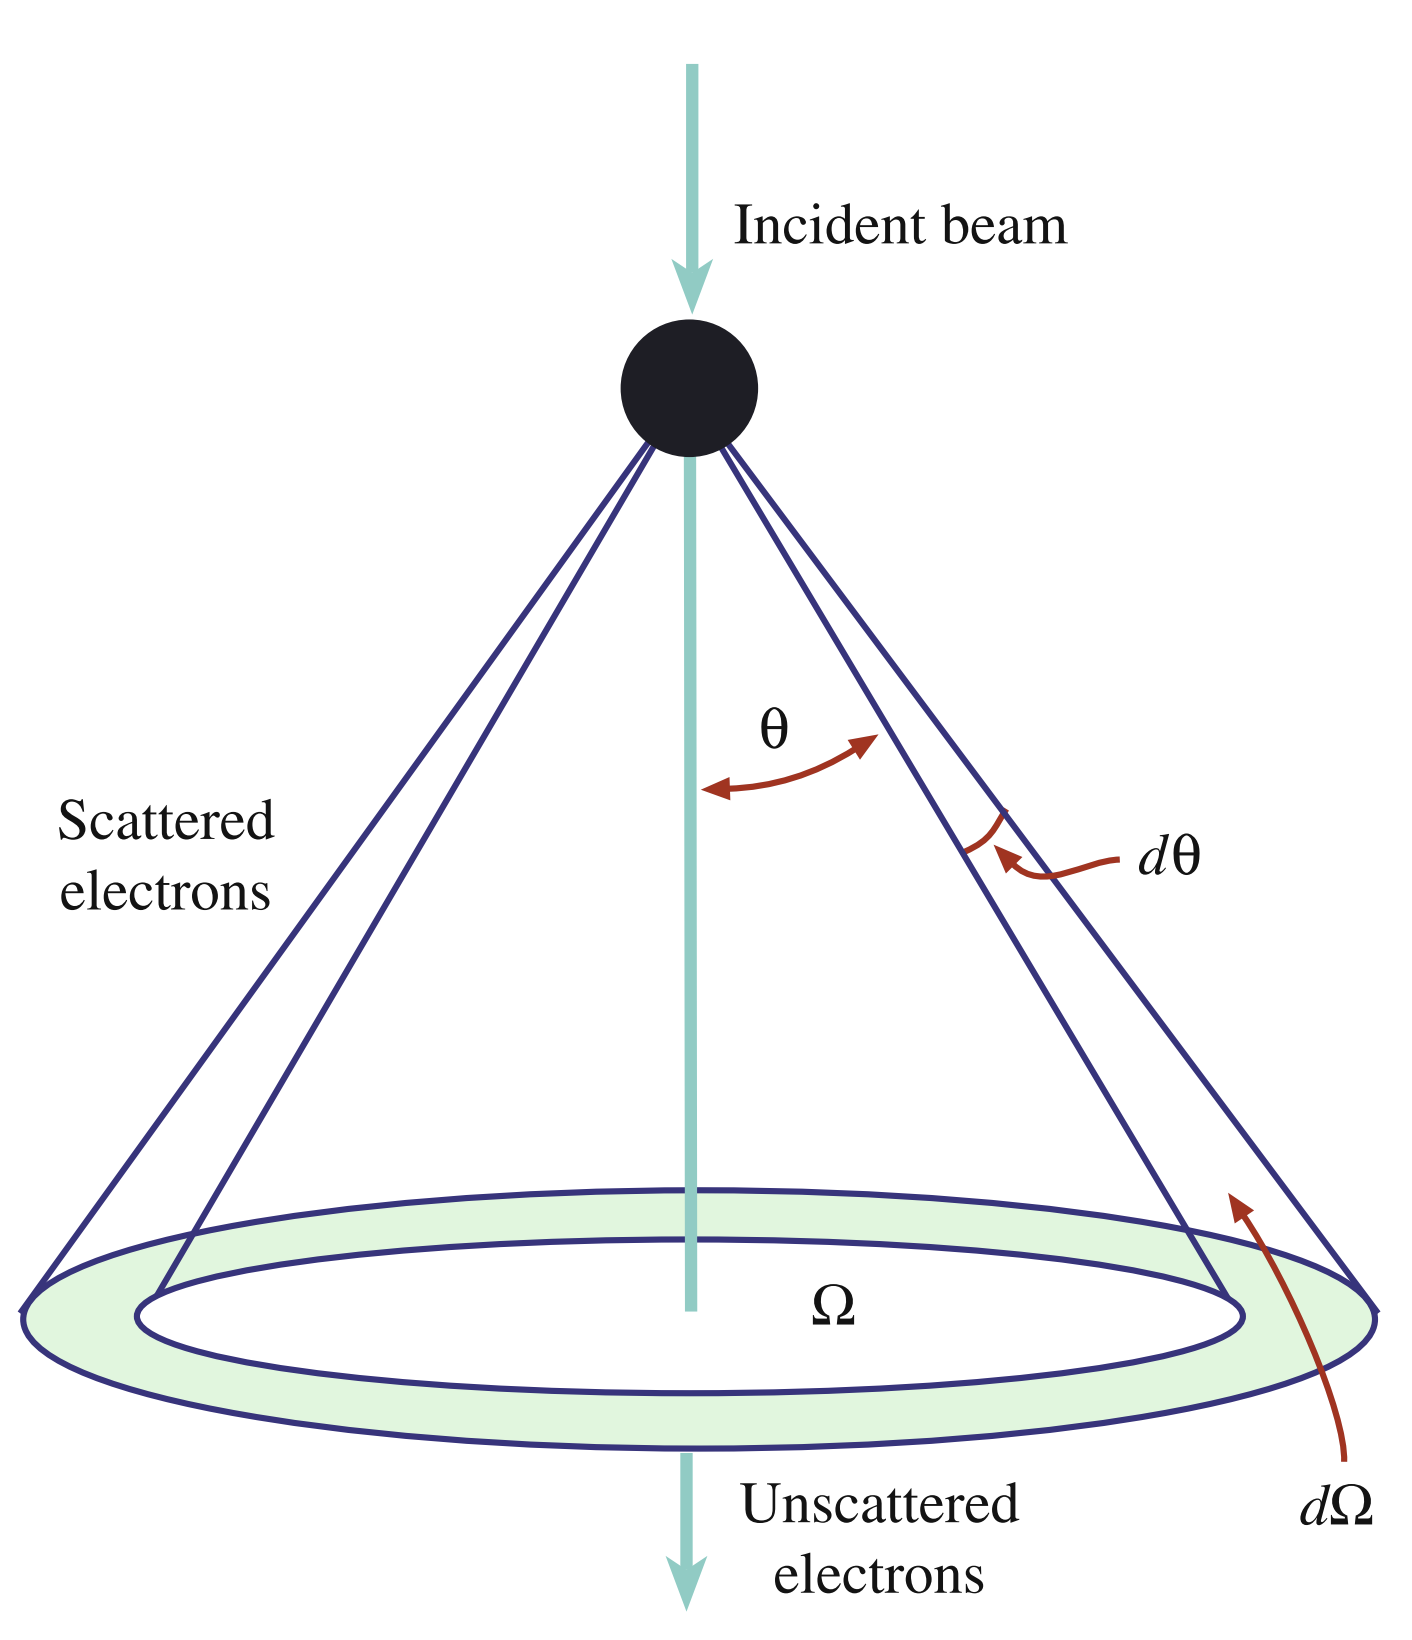
\includegraphics[width=0.5\textwidth]{Chapters/Ch1-Intro/Ch1-Sec1-Background/pics/intro/scattering_geometry.png}
       %     \caption{Geometric relationship between differential scattering angle d$\theta$ and differential solid angle d$\Omega$, from \parencite{Williams2009TransmissionMicroscopy} }
      %      \label{fig:GeometricScattering}
      %  \end{figure}

        \begin{figure}[H]
            \centering
            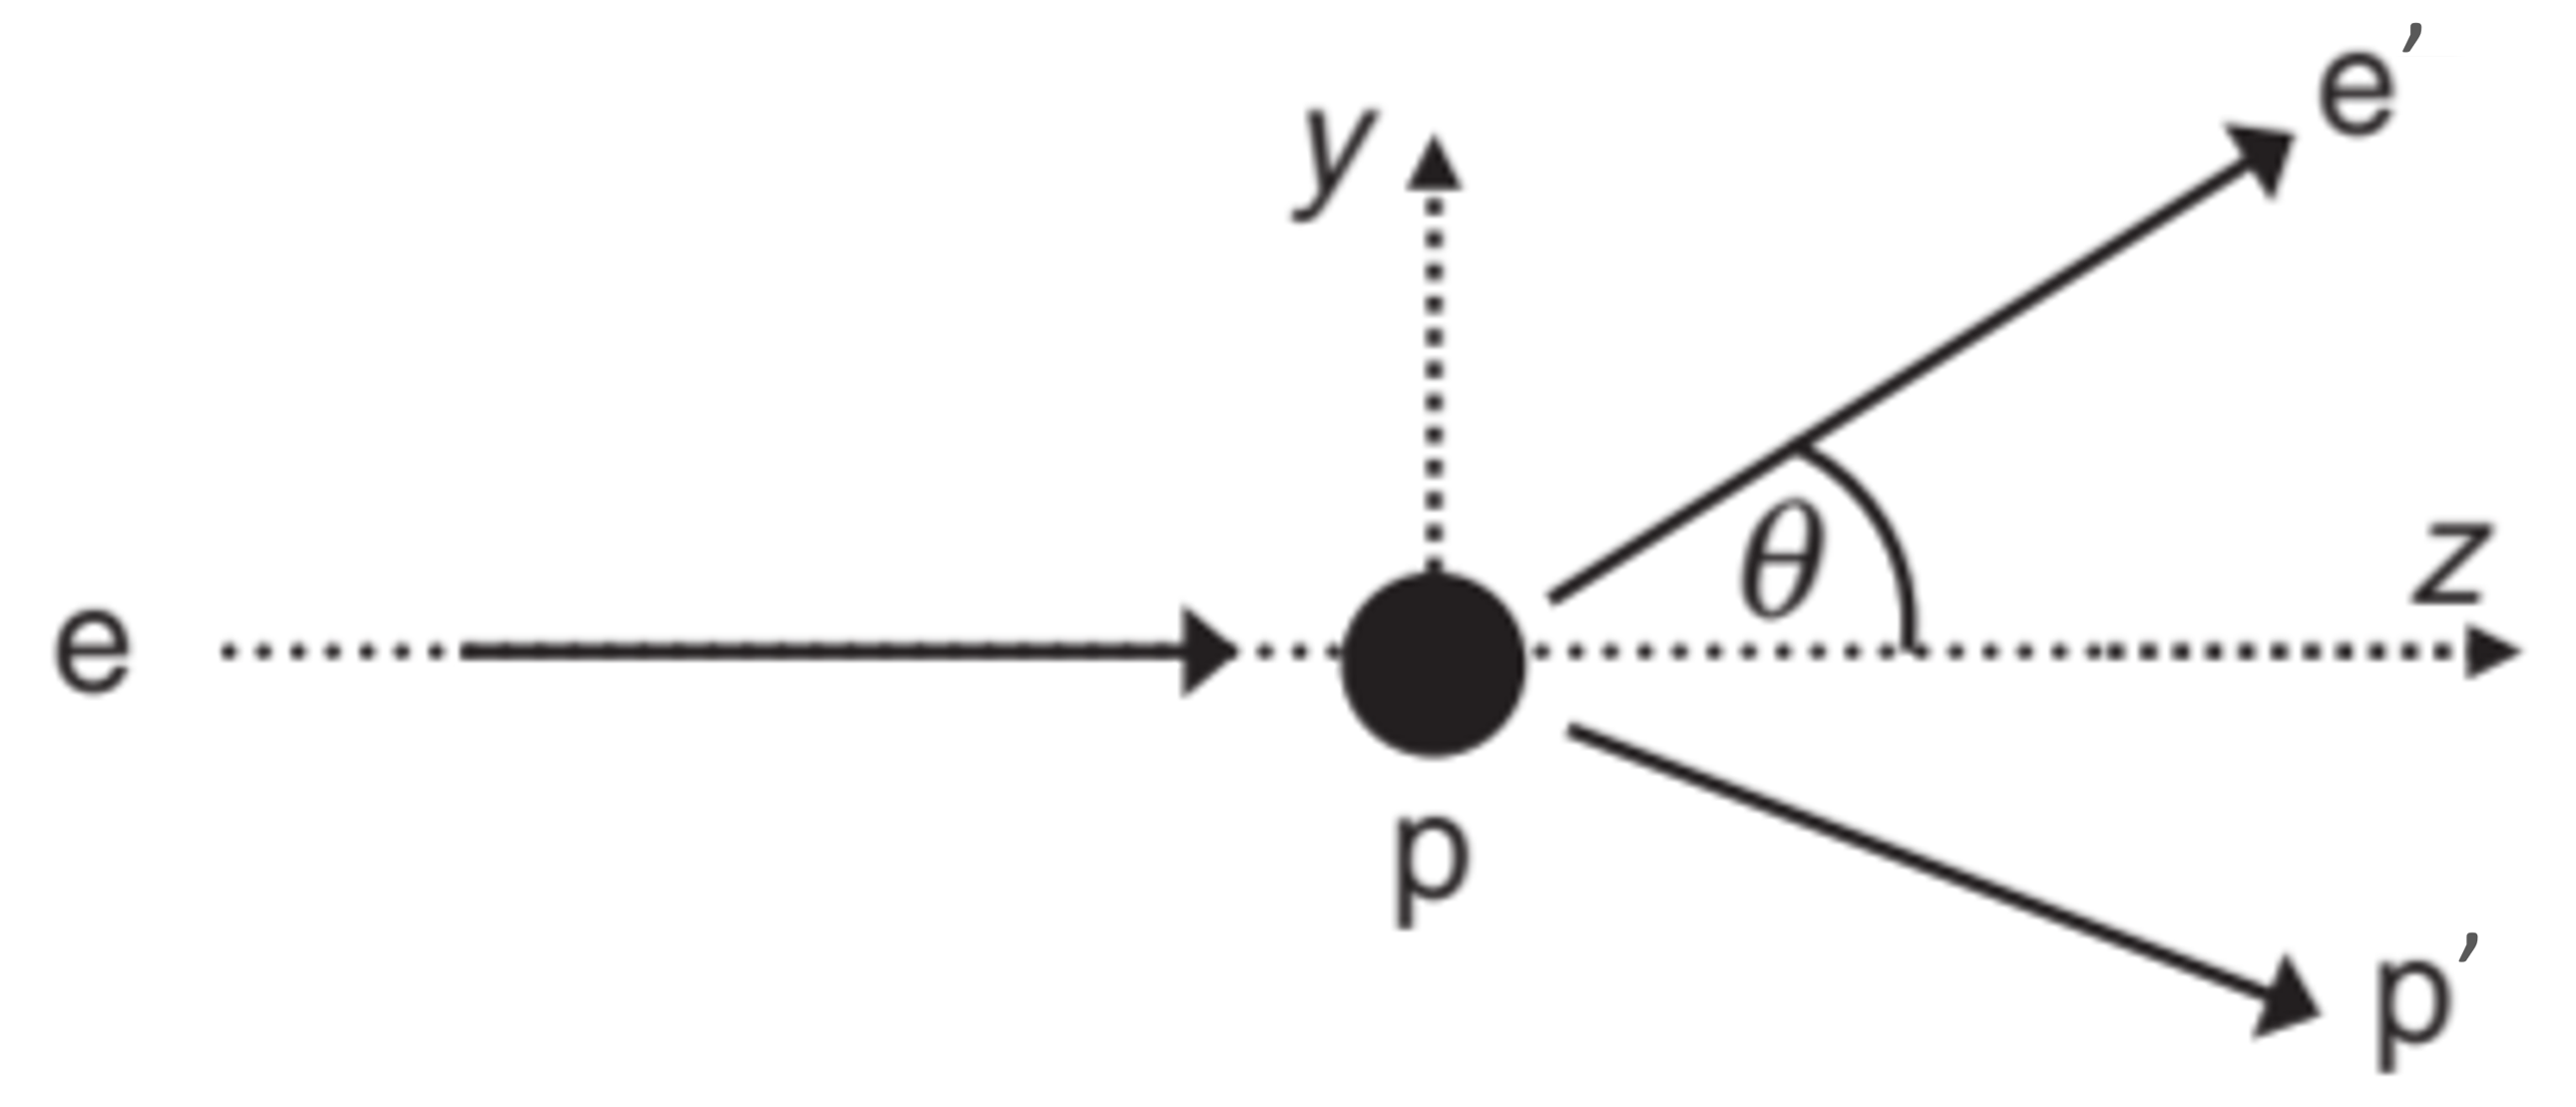
\includegraphics[width=10cm]{Chapters/Ch1-Intro/Ch1-Sec1-Background/pics/elastic-ep/kine-e-2.PNG}
            \caption{Elastic scattering diagram}
        \end{figure}
            
      %  In general, as illustrated in Fig. \ref{fig:GeometricScattering} electrons will scatter through an angle $\theta$ into a solid angle $\Omega$.
        
        
        %as $\Omega = 2\pi(1-\cos{\theta})$, which results in a differential form of $\frac{d\Omega}{d\theta} = 2\pi \sin{\theta}$.

        %From this, we can write the differential cross section as:
        
        %\begin{equation}\label{eq:GeneralDifferentialCrossSection}
        %%   \frac{d\sigma}{d\Omega} = \frac{d\sigma}{d\Omega}\frac{d\Omega}{d\theta} = \frac{1}{2\pi \sin{\theta}}\frac{d\sigma}{d\theta}
        %\end{equation}\myequations{ General Differential Cross Section}


        The scattering cross section for a probe (such as an electron) incident on a target, can be calculated at lowest order by considering a fixed (no recoil), point-like (no structure),  radially symmetric Coulomb potential (e.g., a proton) with a non-relativistic incident charged particle. The resulting equation was used by Rutherford's group in the discovery of the nucleus, and for an electron beam of energy  $E_{beam}$ is given by \eqref{eq:RutherfordDiffX}, where $\alpha$ is the fine structure constant.

            \begin{equation}\label{eq:RutherfordDiffX}
                {\frac{\theta}{2}}(\frac{d\sigma}{d\Omega})_{Ruth} = \frac{\alpha^2}{16E^2_{beam}\sin^4{(\theta/2)}}
            \end{equation}
                \myequations{ Rutherford Scattering Differential Cross Section}

        To probe smaller resolution scales, it is necessary to increase the energy of the beam, and eventually the probe must be treated relativistically. This correction term is provided by the Mott scattering cross section, given by \eqref{eq:MottDiffX}, which still assumes a fixed, point-like target, with only Coulomb interactions.
            
                \begin{equation}\label{eq:MottDiffX}
                     (\frac{d\sigma}{d\Omega})_{Mott} = \frac{\alpha^2}{4E^2\sin^4{(\theta/2)}}\cos^2{\frac{\theta}{2}} = \left( \frac{\alpha}{2E\sin^2{(\theta/2)}}\cos{\frac{\theta}{2}} \right)^2 = 4\cos^2{\frac{\theta}{2}}(\frac{d\sigma}{d\Omega})_{Ruth}
                \end{equation}
                \myequations{ Mott Scattering Differential Cross Section}
        
    
 
         At higher incident electron energies (and thus finer spatial resolutions), the proton's finite size must be accounted for, as well as the momentum transferred to it. The tree-level Feynman diagram for elastic electron-proton scattering is show in in Fig. \ref{fig:feynmanElastic}. The incoming electron \textit{e} exchanges a virtual photon with the proton \textit{p}, resulting in a momentum transfer of $q = p_{e'} - p_{e}$. 
         
        \begin{figure}[H]
            \centering
            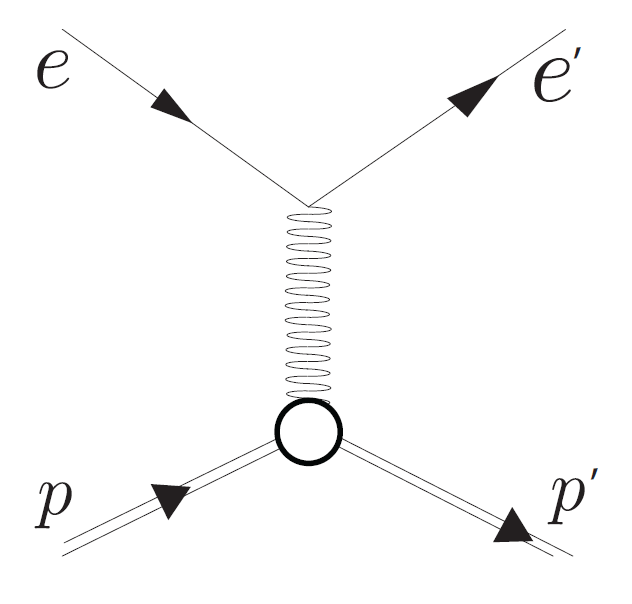
\includegraphics[width=0.5\textwidth]{Chapters/Ch1-Intro/Ch1-Sec1-Background/pics/elastic_feynamn.png}
            \caption{Tree-level elastic scattering Feynman diagram}
            \label{fig:feynmanElastic}
        \end{figure}

        The momentum transfer \textit{q} sets the resolution scale for these processes, but it is convenient to work with the negative square of this value, defined as $Q^2 = -q^2$. With this term, we can express the relativistic differential cross section for the scattering of electrons off a resting, point-like proton as in \eqref{eq:FullElastic}, where $m_p$ is the mass of the proton. 

            \begin{equation}\label{eq:FullElastic}
                    \frac{d\sigma}{d\Omega} = \frac{\alpha^2}{4E_{beam}^2\sin^4{(\theta/2)}} \frac{E_{e'}}{E_{beam}} ( \cos^2{\frac{\theta}{2}} + \frac{Q^2}{2m_p^2}\sin{\frac{\theta}{2}}^2 )
            \end{equation}
            \myequations{ Elastic Scattering Differential Cross Section}


            Compared with Mott Scattering, there are two differences in this formula: The $\frac{E_{e'}}{E_{beam}}$ term in the scattering cross section comes from the electron losing energy to the proton's final state kinetic energy (no longer fixed), and the term proportional to $\sin^2(\theta/2)$ is due to a purely magnetic spin-spin interaction. 


            \indent If the proton were a point, then \eqref{eq:FullElastic} would agree with experiment for all electron scattering energies. Instead, deviations are observed as we increase the beam energy. To account for this structure, we need to include two form factors, $G_E(Q^2)$ - related to the distribution of charge, and $G_M(Q^2)$, related to the distribution of magnetism inside the proton. In the low-$Q^2$ limit, these form factors are the Fourier transforms of the charge an magnetic moment distributions as in \eqref{eq:GE} and \ref{eq:GM}, reducing to the charge and the magnetic moment of the proton in the $Q^2$ = 0 limit. %but the carryover is not exact in general due to being functions of the 4-momenta, instead of 3 momenta. E.g.:

        \begin{equation}\label{eq:GE}
             G_E(Q^2) \approx G_E(q^2) = \int e^{iq\cdot r} \rho (r) d^3r  \quad \quad    G_E(0) = \int  \rho (r) d^3r = 1
        \end{equation}

        \begin{equation}\label{eq:GM}
             G_M(Q^2) \approx G_E(q^2) = \int e^{iq\cdot r} \mu (r) d^3r  \quad \quad  G_M(0) = \int  \mu (r) d^3r = 2.79
        \end{equation}
        
        
        Including these form factors in our cross section gives us the full elastic scattering cross section, as shown in \eqref{eq:rosenbluth}.
                
        \begin{equation}\label{eq:rosenbluth}
            \frac{d\sigma}{d\Omega} = \frac{\alpha^2}{4E_1^2\sin^4{(\theta/2)}}\frac{E_3}{E_1}\left( \frac{G_E^2+\tau G_M^2}{1+\tau} \cos^2{\frac{\theta}{2}}+2\tau G_M^2\frac{Q^2}{2m_p^2}\sin^2(\frac{\theta}{2})\right)
        \end{equation}
       \myequations{ Rosenbluth Scattering Cross Section}
       
        Where $\tau = \frac{Q^2}{4m_p^2}$.
        

        \begin{figure}[H]
            \centering
            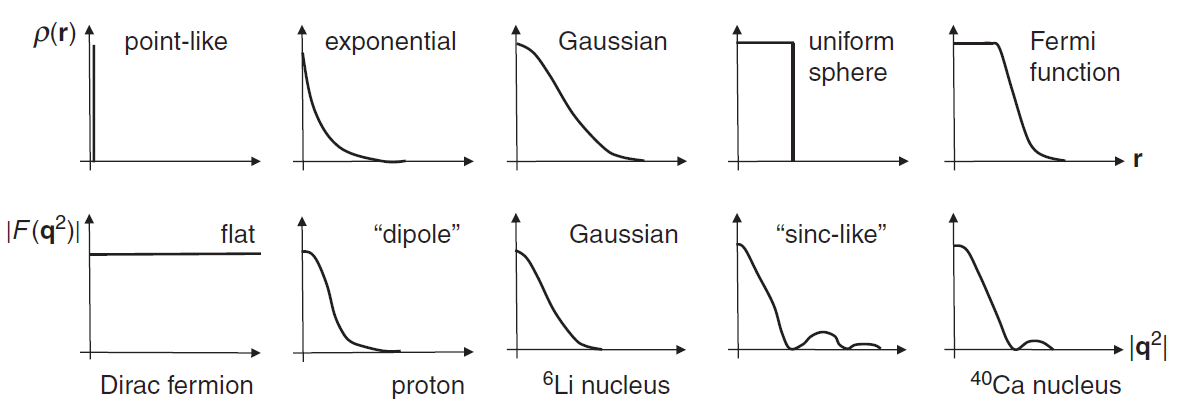
\includegraphics[width=0.9\textwidth]{Chapters/Ch1-Intro/Ch1-Sec1-Background/pics/intro/possibleformfactors.png}
            \caption[Fourier Transforms of Charge Distributions]{Samples of charge distributions and their corresponding form factors $F(\textbf{q}^2)$, from \parencite{Thomson2013ModernPhysics} }
            \label{fig:formfactors}
        \end{figure}
        

                By the 1960s, elastic scattering had been studied sufficiently well as to measure the proton form factors up to several GeV in $Q^2$. The observed results were consistent with a proton having a `dipole' form factor, as shown in Fig. \ref{fig:formfactors}. Investigating proton structure at finer spatial resolutions requires increasing the beam energy, but eventually the the elastic scattering cross section becomes negligible and instead the interactions are sufficiently energetic so as to create additional particles.
                
            %Also something about this is only valid due to angular momentum preservation for 1 photon exchange. 






    \subsection{Inelastic Scattering and Parton Distribution Functions}

        Elastic scattering can be defined as interactions where the target stays intact; specifically, the variable W is the invariant mass of the outgoing struck target \eqref{eq:W}, where elastic scattering satisfies the condition $W^2 =m_p^2$. If $W^2 > m_p^2$, we instead have inelastic scattering, written as ep$\rightarrow$e'X, where X stands for some outgoing hadronic system, as shown in the Feynman diagram in Fig. \ref{fig:FeynmanInelastic}.    

        \begin{equation}\label{eq:W}
            W^2 \equiv (p_p + q)^2 = (p_p + (p_e-p_{e'}))^2
        \end{equation}\myequations{ Outgoing Hadronic System Invariant Mass W}
          

    
        \begin{figure}[ht]
            \centering
            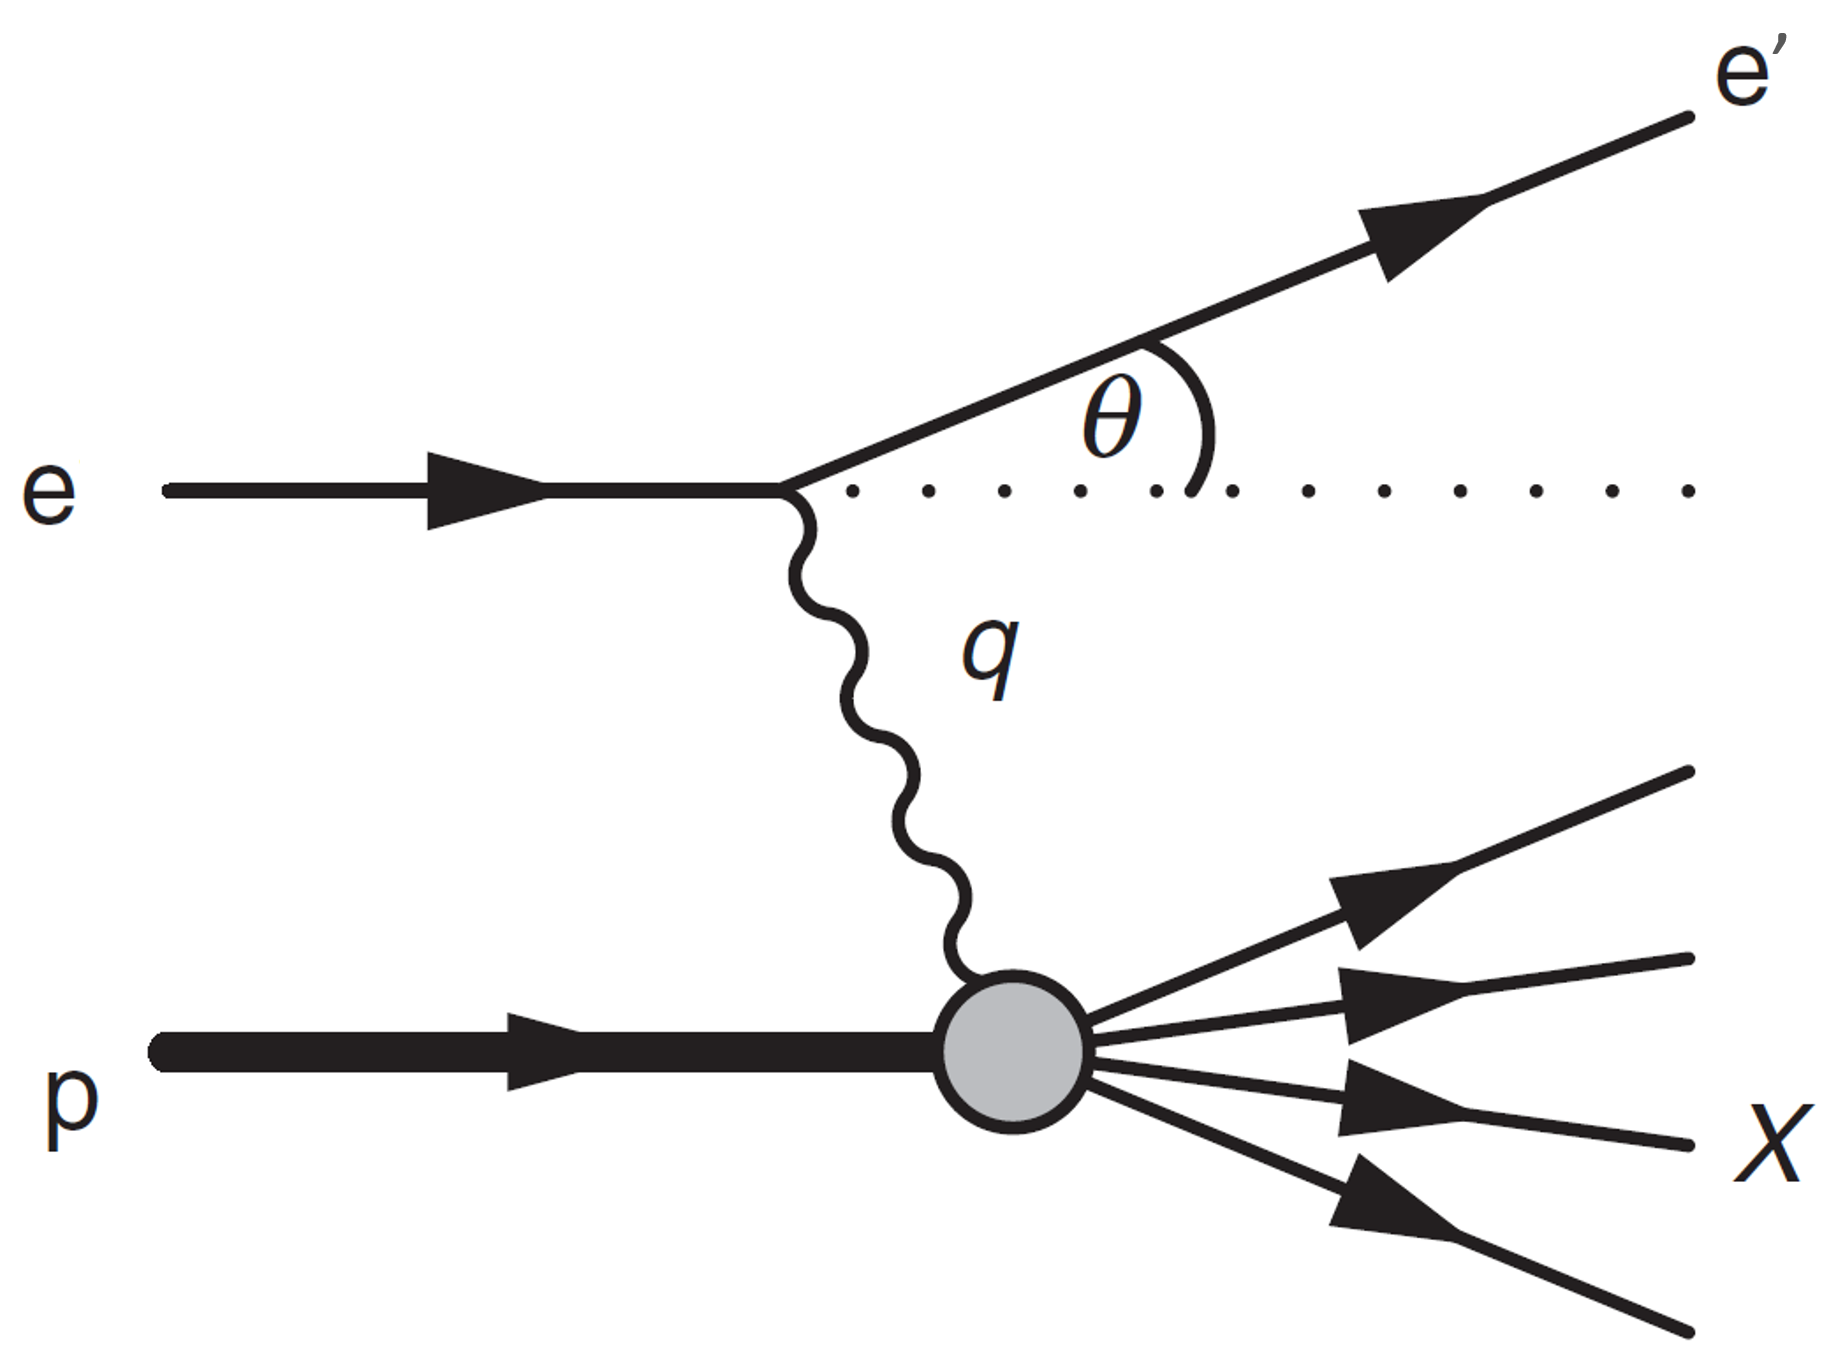
\includegraphics[width=0.6\textwidth]{Chapters/Ch1-Intro/Ch1-Sec1-Background/pics/inelastic-ep/eppx.png}
            \caption{Feynman Diagram for Inelastic Scattering}
            \label{fig:FeynmanInelastic}
        \end{figure}

        The cross section for inelastic scattering has several peaks at various proton resonances, as indicated in the top sketch of Fig. \ref{fig:ScatteringvsW}. Continuing to higher energy transfers we reach the `Deep Inelastic Scattering` (DIS) regime, defined by kinematics as $Q^2$ $>$ 1 GeV$^2$ and W$^2$ $>$4 GeV$^2$. Note that in the DIS process, the proton is smashed apart, yielding many subparticles. Other high-energy inelastic processes where the proton is left intact will be discussed in section \ref{sec:ch1sec2GPDs}. 

        \begin{figure}[ht]
            \centering
            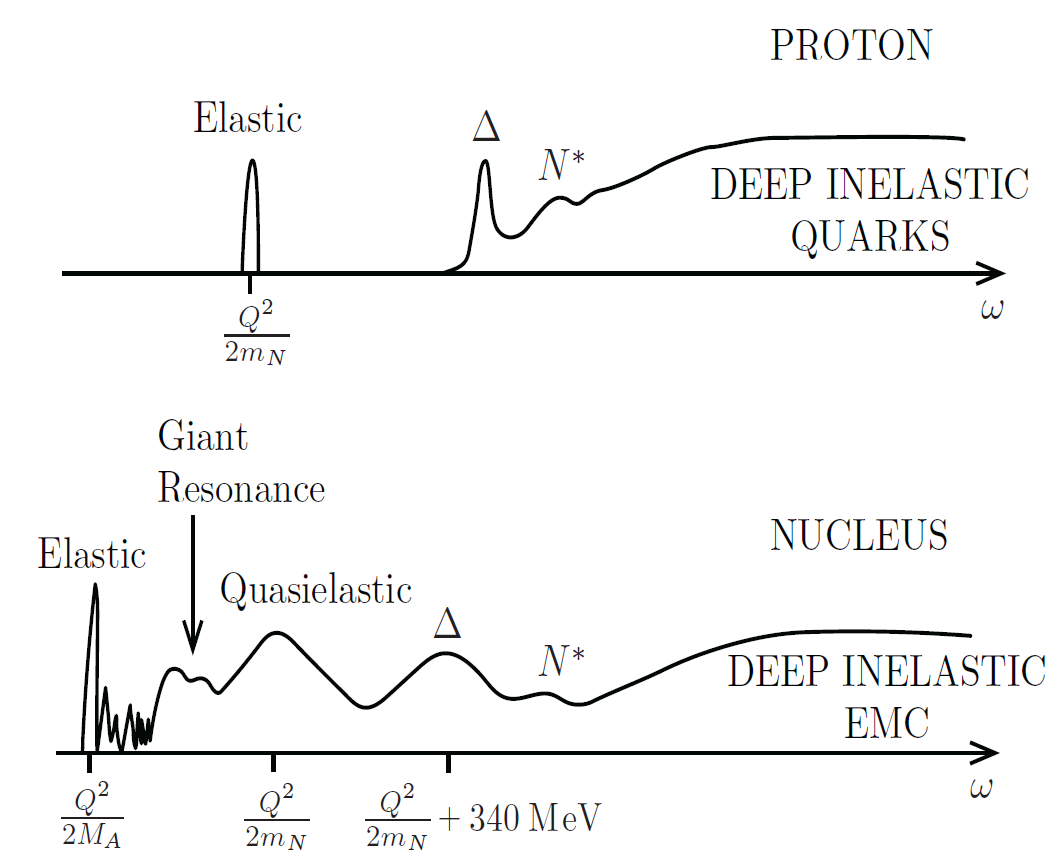
\includegraphics[width=0.6\textwidth]{Chapters/Ch1-Intro/Ch1-Sec1-Background/pics/intro/scatcrosstheory.png}
            \caption[Scattering Cross Section vs. Energy Transfer]{Sketch of cross section as a function of electron energy transfer for inclusive electron scattering off a proton (top) and a nucleus (bottom), from \parencite{Donnelly2017FoundationsPhysics} }
            \label{fig:ScatteringvsW}
        \end{figure}


        Since we remove the constraint that the mass of the final state is the proton mass, we now have one extra degree of freedom, i.e., we need at least 2 variables to describe scattering here. Convenient choices and the squared four-momentum transfer of the virtual photon $Q^2$ and Bjorken X $x_B$, defined in \eqref{eq:xB}. $x_B$ is a measure of elasticity: $x_B$= 1 for elastic scattering. It is useful in that it can also be interpreted as the fraction of proton momentum carried by the struck quark in the infinite momentum frame.       %Think of Xb as the ratio of momentum transfer to energy transfer. 

        \begin{equation}\label{eq:xB}
            x_B \equiv \frac{Q^2}{2p_p\cdot q} = \frac{Q^2}{Q^2+W^2-m_p^2}
        \end{equation}\myequations{ Bjorken X}


        Another useful quantity is \textit{y}, which is a measure of the inelasticity of the scattering. It is the fractional energy lost by the electron in the scattering process, where y=0 is for perfectly elastic collisions, and is given by \eqref{eq:y}
        
        \begin{equation}\label{eq:y}
            y \equiv \frac{p_p \cdot q}{p_p \cdot p_e} = \frac{\nu}{E_{beam}} =  1 - \frac{E_{e'}}{E_{beam}} 
        \end{equation}\myequations{ Inelasticity y}

        Where $\nu$ is the energy transferred in the collision \eqref{eq:nu}. 
        \begin{equation}\label{eq:nu}
            \nu = \frac{Q^2}{2*x_B*m_p}
        \end{equation}\myequations{ Energy Transfer $\nu$}
        

        With these definitions, we can write the differential cross section for inelastic scattering. Note that the general formula for the differential cross section for elastic scattering, \eqref{eq:rosenbluth} can be re-written in explicitly Lorentz-invariant form as in \eqref{eq:rosen-lorentz}.
        %as shown in \eqref{eq:InelasticDiffCross}

        \begin{equation}\label{eq:rosen-lorentz}
            \frac{d\sigma}{d\Omega} = \frac{4\pi\alpha^2}{Q^4} \left[ \left( 1 -y -\frac{m_p^2 y^2}{Q^2}       \right) \frac{G_E^2+\tau G_M^2}{1+\tau} +y^2 \frac{G_M^2}{2} \right]
        \end{equation}
       \myequations{ Lorentz-invariant Rosenbluth Scattering Cross Section}

        This equation can be generalized to extend to inelastic scattering by replacing the terms corresponding to the combinations of form factors $G_E$ and $G_M$ with more structure functions $F_1(x_B,Q^2)$ and $F_2(x_B,Q^2)$, which describe proton structure as a function of both independent variables. This results in the differential cross section given by \eqref{eq:fullinelastic} .

        \begin{equation}\label{eq:fullinelastic}
            \frac{d\sigma}{d\Omega} = \frac{4\pi\alpha^2}{Q^4} \left[ \left( 1 -y -\frac{m_p^2 y^2}{Q^2}       \right) \frac{F_2(x_B,Q^2)}{x_B} +y^2 F_1(x_B,Q^2) \right]
        \end{equation}
       \myequations{  Scattering Cross Section in Terms of $F_1(x_B,Q^2)$ and $F_2(x_B,Q^2)$}


        %\textcolor{red}{input stuff about standard model, what is a pion, electron, proton, photon}\mytodo{standard model information}
        \todo{input standard model, pion information}
        
        Experiments in the 1960s on DIS indicated that the structure functions $F_1(x_B,Q^2)$ and $F_2(x_B,Q^2)$ were nearly independent of $Q^2$, a feature known as Bjorken scaling \parencite{Bjorken1969InelasticNucleon}. This indicated scattering was occurring off of point-like constituents - current experiment results provide a constraint on the maximum radius of these constituent to be at most $10{-18}$ m \parencite{Thomson2013ModernPhysics}. 


        Secondly, DIS results indicated the two structure functions could be expressed as $F_2(x_B) = 2*x_B*F_1(x_B)$, named the Callan-Gross relation. This relationship can be explained if the electron is scattering off of spin-half point-like particles inside the proton, which combined with Bjorken scaling to given strong evidence for the existence of quarks inside the proton, and gave motivation for the development of the parton model \parencite{Feynman1969VeryHadrons}.

        
        
        The parton model connects the experimentally measurable structure functions to Parton Distribution functions which describe the distribution of proton longitudinal momentum amongst its constituents. Specifically, a PDF $q_i(x_B)$ describes the probability density of finding a parton carrying a longitudinal momentum fraction in the interval ($x_B$, $x_B + dx_B$). The relationship between PDFs and structure functions is given by \eqref{eq:PDFs}, where $Q_i$ is the charge of each quark.

        \begin{equation}\label{eq:PDFs}
            F_2^p(x_B) = x_B \sum_i Q^2_i q_i(x_B)
        \end{equation}
       \myequations{ $F_2$ structure function in terms of PDFs}
        
        Structure functions have been studied in great detail over a very large kinematic range across $Q^2$ and $x_B$, the results of which are shown in Fig. \ref{fig:HERA}.
        %up to $Q^2 = 20,000 GeV^2$ and $x < 0.0001$. $Q^2$     
    
        
        \begin{figure}[H]
            \centering
            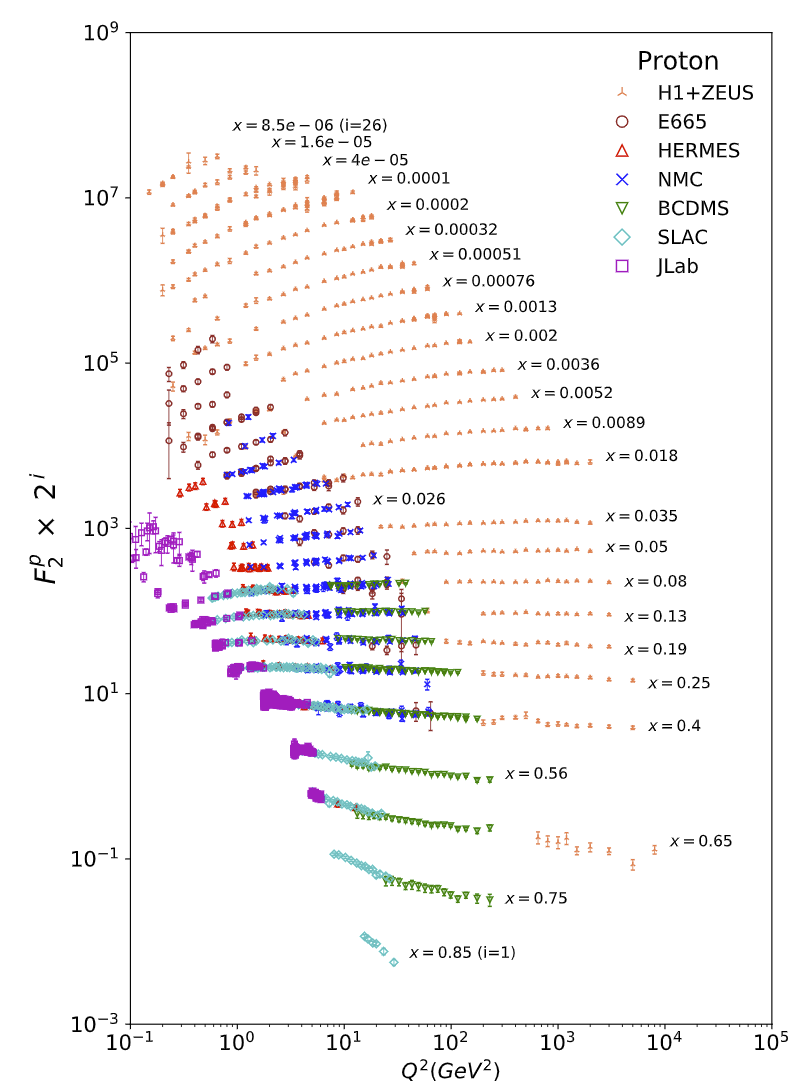
\includegraphics[width=0.6\textwidth]{Chapters/Ch1-Intro/Ch1-Sec1-Background/pics/inelastic-ep/protF2.png}
            \caption[Proton Structure Function $F^p_2$]{The proton structure function $F^p_2$, measured at various experiments as listed, all with $W^2>3.5 GeV^2$. $F^p_2$ values have been multiplied by 2$^{ix}$ for visual purposes, from \parencite{Zyla2020ReviewPhysics}}.
            \label{fig:HERA}
        \end{figure}

        The global experimental results can be combined with theoretical QCD frameworks such as the DGLAP evolution equations \parencite{Altarelli1977AsymptoticLanguage}. to plot PDFs for various constituents of the proton, as shown in Fig. \ref{fig:PDFPlots}. 
        
                \begin{figure}[H]
            \centering
            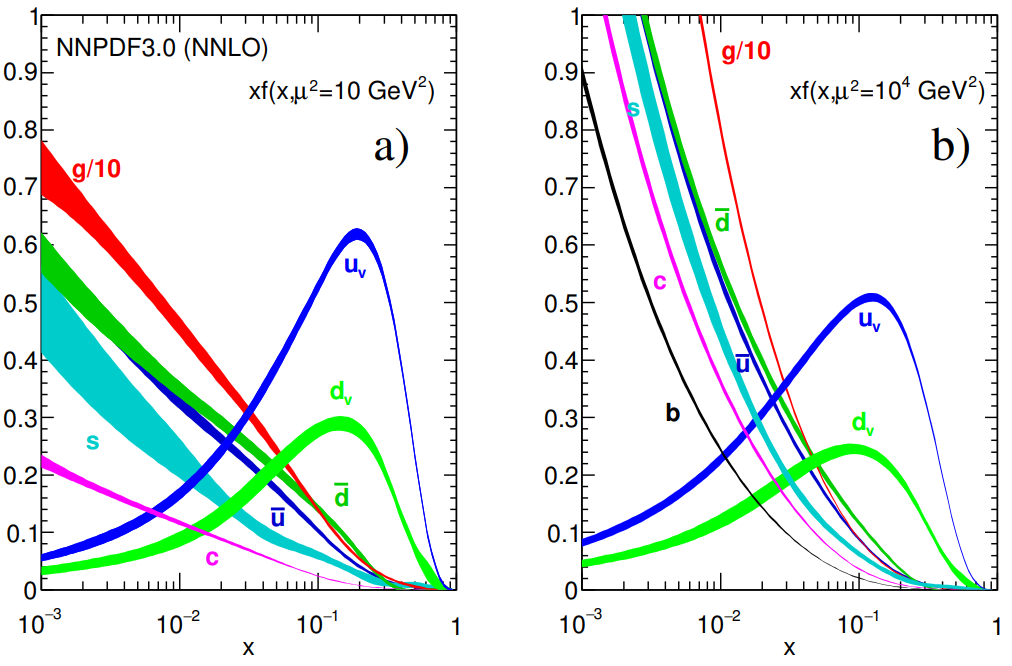
\includegraphics[width=0.7\textwidth]{Chapters/Ch1-Intro/Ch1-Sec1-Background/pics/inelastic-ep/partonPDFs.png}
            \caption[Parton Distribution Functions]{Quark and gluon distribution functions from NNLO NNPDF3.0 global analysis at $\mu^2$= 10 GeV$^2$ (left) and $\mu^2$= 10$^4$ GeV$^2$ (right),  from \parencite{Zyla2020ReviewPhysics}}
            \label{fig:PDFPlots}
        \end{figure}

       All of these major scattering scales explored through the 20$^{th}$ century are summarized in \figref{fig:experimentsVsscale}, spanning roughly four orders of magnitude in length scale. While steady increases in resolving power have been made, the focus of this work (red triangle in figure) is not to image even finer scale parton dynamics, but rather to understand the multidimensional structure of the nucleon. In particular, while PDFs allow for a 1 dimensional mapping of the inner workings of a proton, even more information can be gleaned from more complex scattering reactions. Efforts are now directed towards so called \textit{proton tomography} - 3D imaging of nucleon structure - which is the focus of this analysis. 

        \begin{figure}
            \centering
            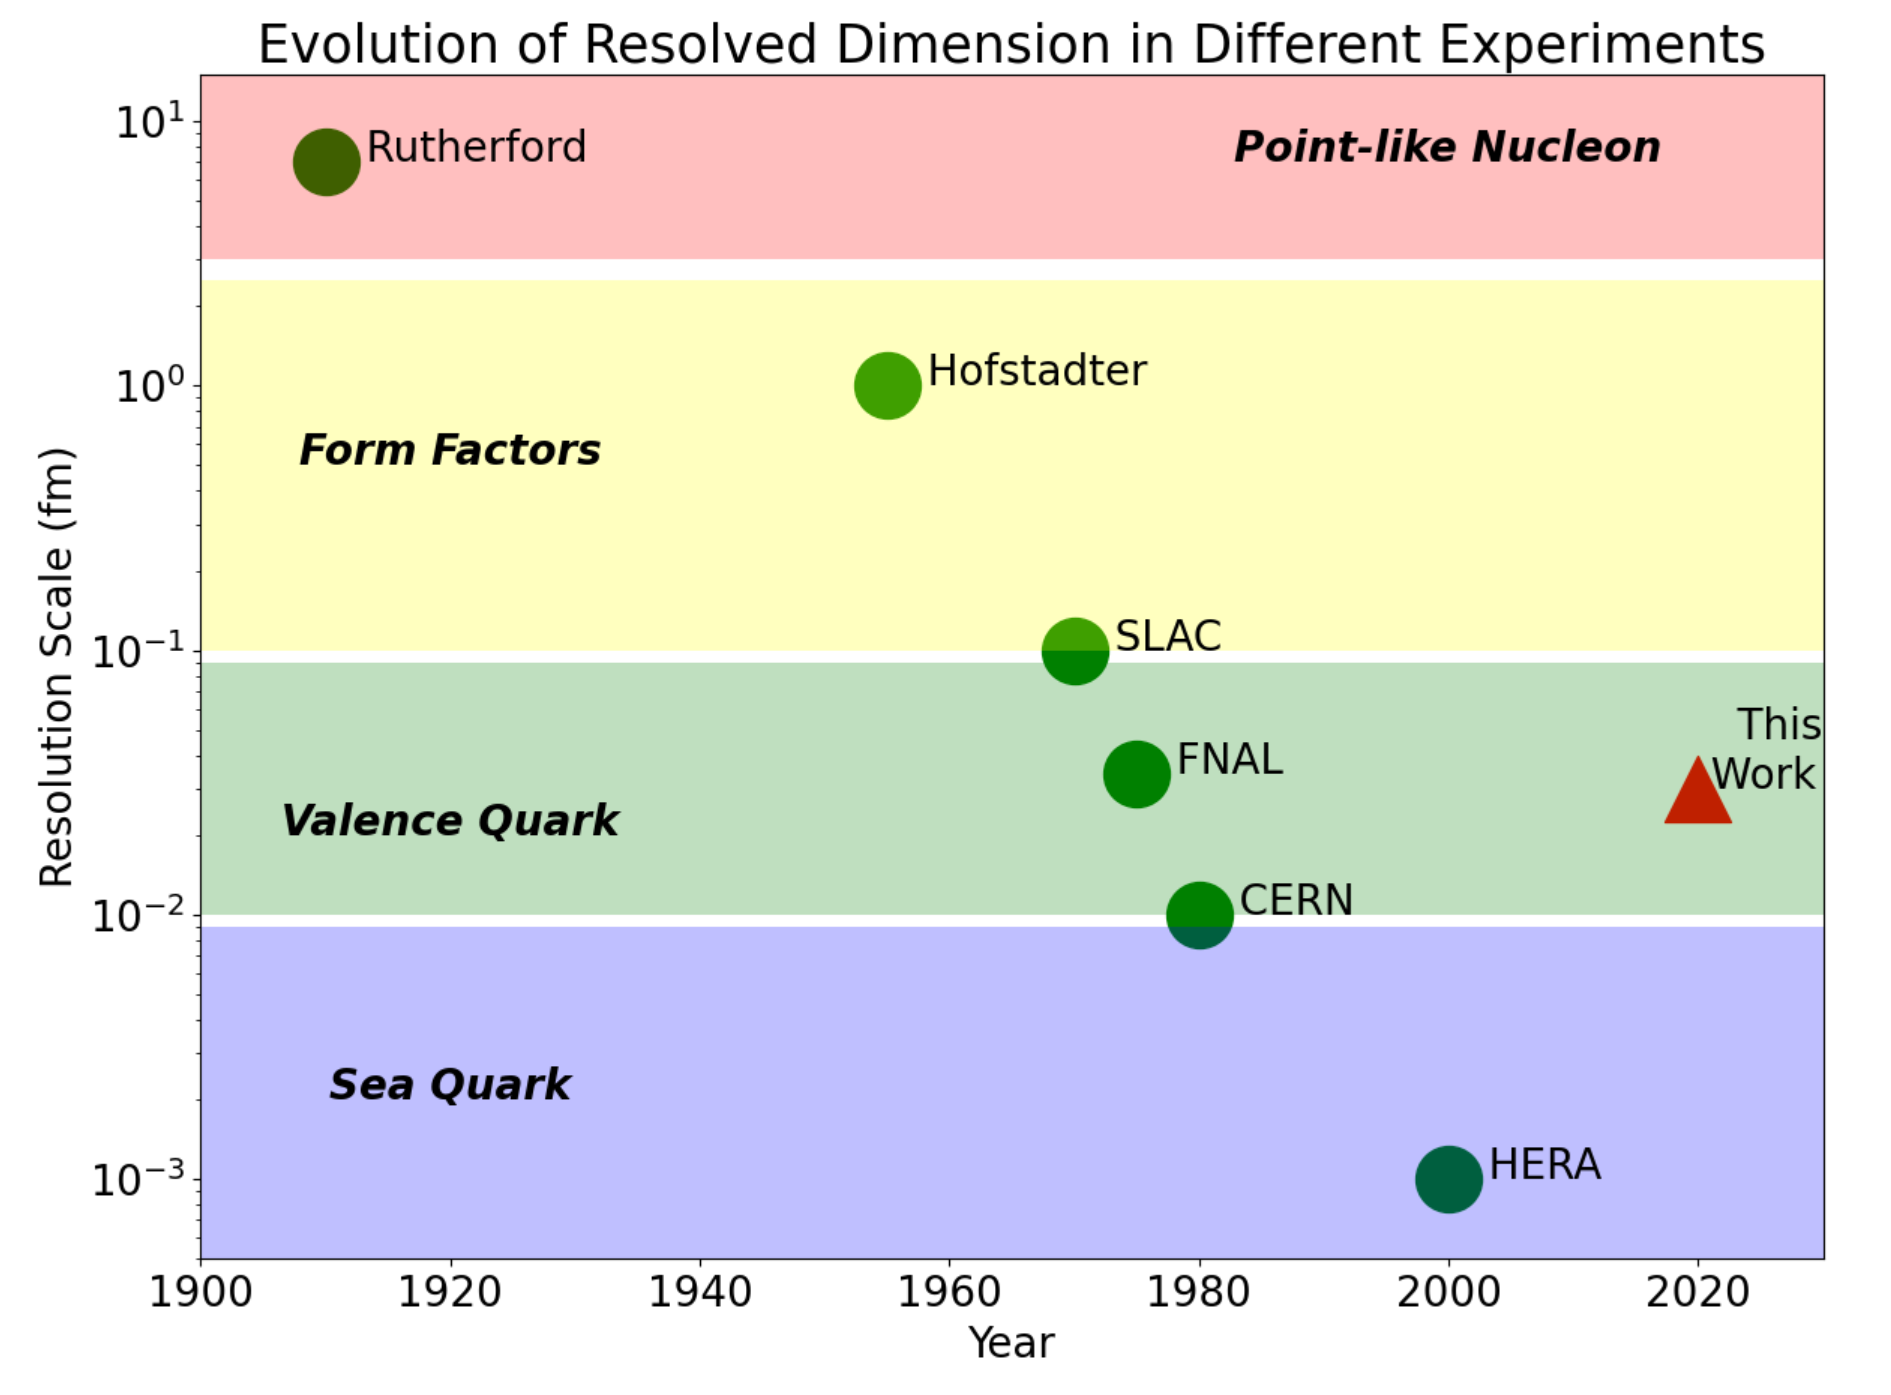
\includegraphics[width=0.9\textwidth]{Chapters/Ch1-Intro/Ch1-Sec1-Background/pics/experiment_scales.png}
            \caption[Scattering Measurements at Different Scales]{Scattering experiments performed at different energy scales reveal different information about proton structure. This work (red triangle) focuses on multi-dimensional structure mapping in the valence quark regime. Figure modified from \parencite{Klein2005ResolvingHERA}}.
            \label{fig:experimentsVsscale}
        \end{figure}





\iffalse
       \subsection{Deviation into Rosenbluth and TPEX}
        
                
            The Rosenbluth method of measuring the ratio of $G_E$ and $G_M$ has awful systematics, based mainly in the facts that you need to measure an absolute cross section, worry about radiative corrections, and measure at low $Q^2$. A better way to measure the proton form factor ratio is by a \textbf{polarization transfer} measurement. This uses a \textbf{Focal Plane Polarimeter} to converst transverse polarization into an azimuthal distribution:
            
                  
            \begin{figure}[H]
                \centering
                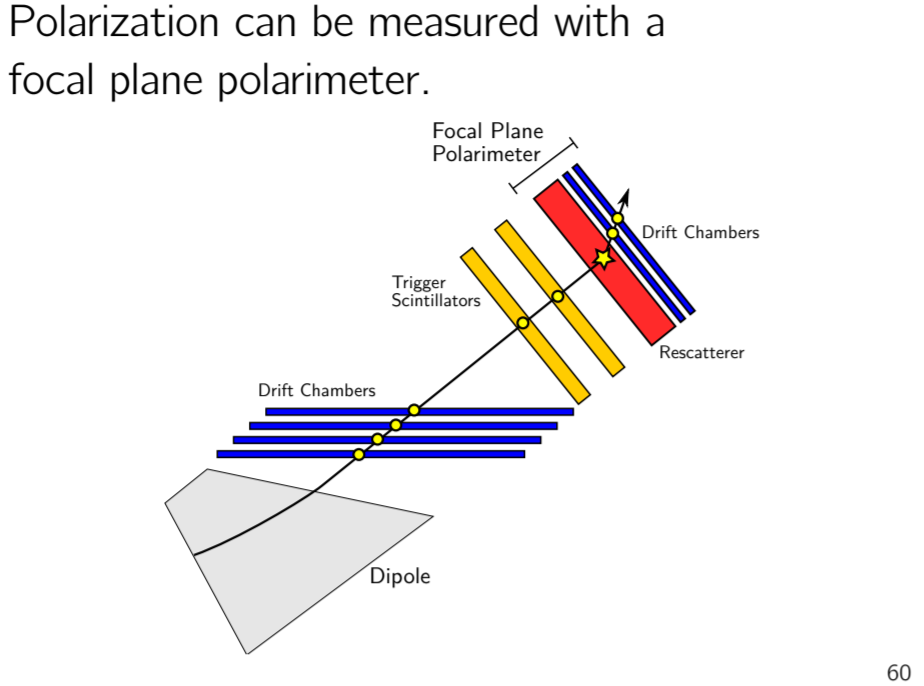
\includegraphics[width=10cm]{Chapters/Ch1-Intro/Ch1-Sec1-Background/pics/elastic-ep/olympus-fpp.PNG}
                \caption{Olympus experimental setup}
            \end{figure}
            
            This method has the advantages that we are measuring a ratio, not an absolute cross section, so many uncertainties cancel, such as the FPP analyzing power. Olympus produced the following:
            
                  
            \begin{figure}[H]
                \centering
                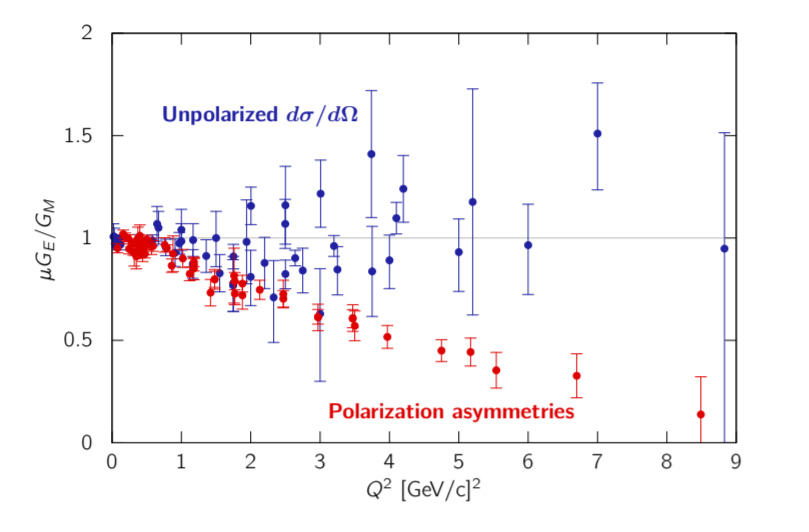
\includegraphics[width=10cm]{Chapters/Ch1-Intro/Ch1-Sec1-Background/pics/elastic-ep/olympus-form-factors.PNG}
                \caption{$G_E$ and $G_M$ ratio measurements}
            \end{figure}
            
            This discrepancy may be due to two photon exchange, which we can measure by comparing electron to positron scattering:
            
                  
            \begin{figure}[H]
                \centering
                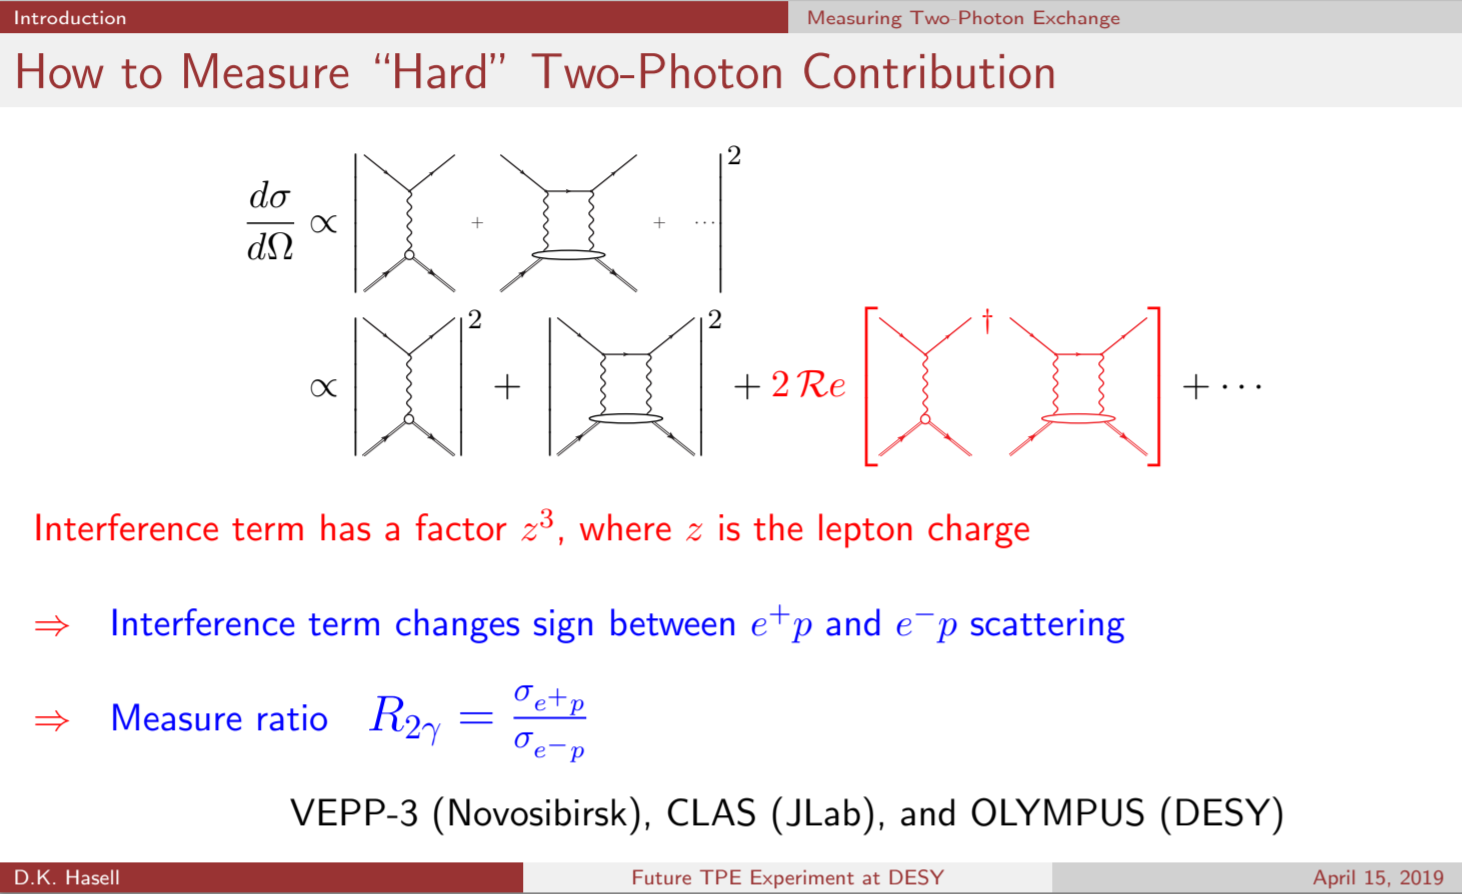
\includegraphics[width=10cm]{Chapters/Ch1-Intro/Ch1-Sec1-Background/pics/elastic-ep/tpex.PNG}
                \caption{Electron Positron charge interference}
            \end{figure}
        
        
            TPEX is a currently proposed experiment to extend this out to farther $Q^2$, which is challenging due to its lower luminosity of elastic scattering as $Q^2$ increases.    

            Alarcon's 2023 study discusses the two-photon exchange experiment TPEX \parencite{Alarcon2023Two-PhotonTPEX}.

\fi




   \iffalse


           \begin{figure}[H]
            \centering
            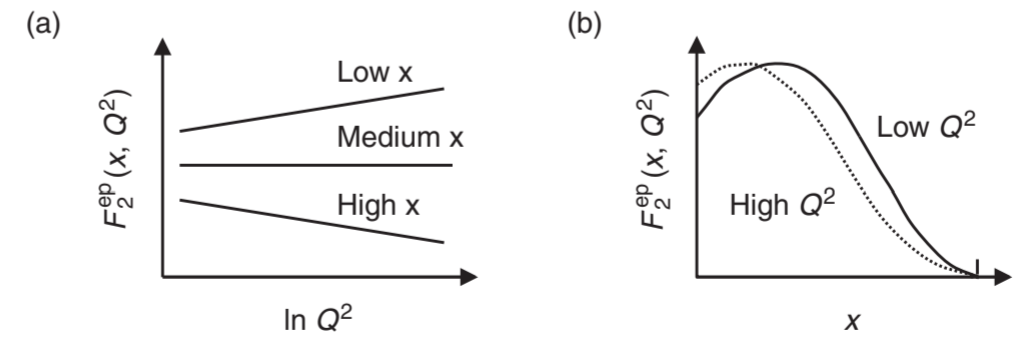
\includegraphics[width=12cm]{Chapters/Ch1-Intro/Ch1-Sec1-Background/pics/inelastic-ep/scaling-violations.PNG}
            \caption{Explanation of Scaling Violations}
        \end{figure}
        


        \indent These describe the distribution of quarks within the nucleon. Describes the momentum fraction distribution of quarks. For example:\\
        \newline
        $u^p(x)dx$\\
        \newline
        Represents the number of up-quarks within the proton with momentum fraction between x and dx. The functional forms of the PDFs are not a-priori known. Some potential PDFs could be as shown below:\\

        \begin{figure}[H]
            \centering
            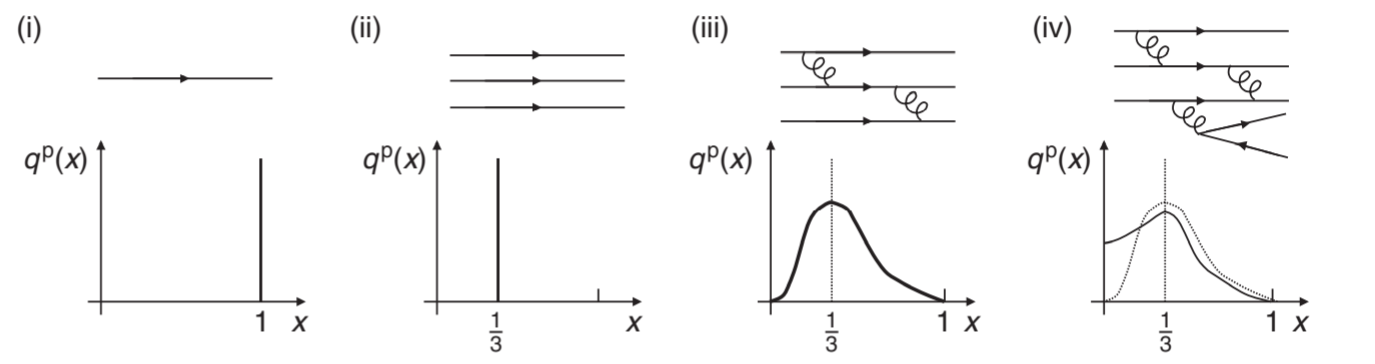
\includegraphics[width=12cm]{Chapters/Ch1-Intro/Ch1-Sec1-Background/pics/inelastic-ep/pdf-possibilities.PNG}
            \caption{Potentail PDFs}
        \end{figure}
        
        (i) - if the proton consisted of a single quark\\
        (ii) - if the proton had 3 static quarks\\
        (iii) - quarks interacting and Heisenberg uncertainty (momentum smearing)\\
        (iv) - interacting quarks with higher order diagrams - gluons produced, so enhances low x part of PDF\\
        \newline
        We can access these distributions experimentally as the parton model predicts the the cross section for elastic scattering off of quarks with charge $Q_i$ and momentum fraction in the range of x to x + dx as:
        \fi